\bookmarksetup{startatroot}
\chapter*{List Of Exercises}
\addcontentsline{toc}{chapter}{List Of Exercises}

\section*{\nameref*{chap:linear-systems}}

\begin{enumerate}
 \item Solve each of the systems below using matrix notation. Write the solution
  in the form of \myref{theorem}{thm:solution-set-of-a-linear-system}.
  \[
   \begin{array}[t]{r c r c r}
    3x & + & 6y & = & 18\\
    x & + & 2y & = & 6
   \end{array} \hspace{2em}
   \begin{array}[t]{r c r c r}
    x & + & y & = & 1\\
    x & - & y & = & -1
   \end{array} \hspace{2em}
   \begin{array}[t]{r c r c r c r c r}
    x_1 & + & 2x_2 & - & x_3 & & & = & 3\\
    2x_1 & + & x_2 & & & + & x_4 & = & 4\\
    x_1 & - & x_2 & + & x_3 & + & x_4 & = & 1
   \end{array}
  \]
 \item Show that any five points in the plane $\R^2$ lie on a common \emph{conic
  section}, that is, they all satisfy an equation of the form
  \[
   ax^2 + by^2 + cxy + dx + ey + f = 0
  \]
  for some $a,\ldots,f \in \R$.
 \item 
 Prove that if $\mathbf{s}$ and $\mathbf{t}$ are solutions of a homogeneous
 linear system, then so are
 \begin{enumerate}
  \item $\mathbf{s} + \mathbf{t}$,
  \item $3 \mathbf{s}$,
  \item $k \mathbf{s} + m \mathbf{t}$ for any numbers $k,m$.
 \end{enumerate}
 What is wrong with the following argument: `These three show that if a
 homogeneous system has one solution, then it has many solutions -- any multiple
 of a solution is another solution, and any sum of solutions is also a solution
 -- so there are no homogeneous linear systems with exactly one solution.'?
\item 
 Find examples of linear systems of three equations in two variables that
 correspond to parts (b) and (d) of \myref{figure}{fig:arrangement-of-lines}.
\item 
 Draw the following linear systems.
 \[
  \begin{array}{r c r c r}
   2x & + & y & = & 1\\
   3x & + & 2y & = & 3
  \end{array}
  \hspace{3em}
  \begin{array}{r c r c r}
   -x & + & y & = & 2\\
   2x & - & 2y & = & 5
  \end{array}
  \hspace{3em}
  \begin{array}{r c r c r}
   -x & - & y & = & 1\\
   3x & + & 2y & = & 0
  \end{array}
 \]
\item 
 Without depicting them visually, determine the arrangement of planes
 corresponding to the linear system below.
 \[
  \begin{array}{r c r c r c r}
   2x & - & y & + & z & = & 3\\
   x & - & 3y & + & 4z & = & 1\\
   x & + & 2y & - & 3z & = & 2
  \end{array}
 \]
\item 
 Find linear systems in three variables and three equations corresponding to
 cases (1), (4) and (5) in the text above.
\item 
 Show that transformations (1) and (2) also don't change the set of solutions of
 the transformed linear system.
\item 
 Using \emph{Gauss-Jordan elimination} solve the systems from
 examples~\ref{exam:static-equations} and~\ref{exam:chemical-reactions}.
\item 
 Use Gauss-Jordan elimination to solve the following system.
 \[
  \begin{array}{r c r c r c r}
   x_1 & &  & - & x_3 & = & 0\\
   3x_1 & + & x_2 & & & = & 1\\
   -x_1 & + & x_2 & + & x_3 & = & 4
  \end{array}
 \]
\item 
 Each of the following systems is in echelon form. Determine their number of
 solutions (without calculation).
 \begin{center}
  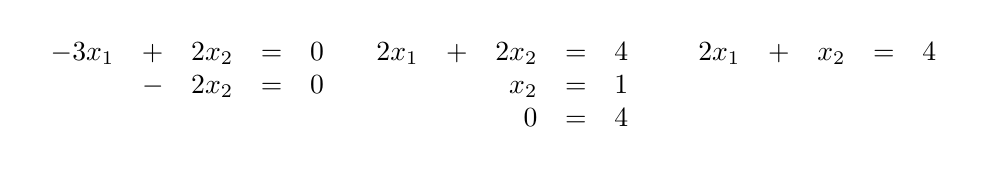
\begin{tikzpicture}
   \node at (0,0) {$
    \begin{array}{r c r c r}
     2x_1 & + & 2x_2 & = & 4\\
      & & x_2 & = & 1\\
       & & 0 & = & 4
    \end{array}
    $};
   \node at (-4,0) {$
    \begin{array}{r c r c r}
     -3x_1 & + & 2x_2 & = & 0\\
      & - & 2x_2 & = & 0\\
      & & & &
    \end{array}
    $};
   \node at (4,0) {$
    \begin{array}{r c r c r}
     2x_1 & + & x_2 & = & 4\\
      & & & &\\
      & & & &
    \end{array}
    $};
  \end{tikzpicture}
 \end{center}
\item 
 Find the values of $a,b$ and $c$ that cause the graph of $f(x) = ax^2 + bx + c$
 to pass through the points $(1,2)$, $(-1,6)$ and $(2,3)$.
\item 
 Show that for all numbers $a,b,c,d,j,k$ such that $ad - bc \neq 0$, the system
 \[
  \begin{array}{r c r c r}
   ax_1 & + & bx_2 & = & j\\
   cx_1 & + & dx_2 & = &k
  \end{array}
 \]
 has a \emph{unique} solution.
\end{enumerate}

\section*{\nameref*{chap:linear-geometry}}

\begin{enumerate}
 \item 
 Describe the plane passing through points $(1,1,5,-1)$, $(2,2,2,0)$ and
 $(3,1,0,4)$ as
 \begin{enumerate}[label=(\alph*)]
  \item a set of points,
  \item a set of vectors.
 \end{enumerate}
 Does the origin $(0,0,0,0)$ lie in the plane?
\item 
 Describe the plane (as a set of points or vectors, as you wish) that contains
 \[
  \text{the point }
  \begin{pmatrix}
   2\\
   0\\
   3
  \end{pmatrix}\text{ and the line }
  \left\{\begin{pmatrix}
   1\\
   1\\
   0
  \end{pmatrix}
  + t
  \begin{pmatrix}
   1\\
   1\\
   2
  \end{pmatrix}
  \mid t \in \R \right\}.
 \]
\item 
 A person travelling eastward at a rate of 3 miles per hour finds that the wind
 appears to blow directly from the north. On doubling his speed it appears to
 come from the north east. What was the wind's velocity?
\item 
 Find the length of each of the vectors
 \[
  \begin{pmatrix}
   3\\
   1
  \end{pmatrix}, \quad 
  \begin{pmatrix}
   -1\\
   2
  \end{pmatrix}, \quad 
  \begin{pmatrix}
   4\\
   1\\
   1
  \end{pmatrix}, \quad 
  \begin{pmatrix}
   0\\
   0\\
   0
  \end{pmatrix}, \quad \text{and} \quad 
  \begin{pmatrix}
   1\\
   -1\\
   1\\
   0
  \end{pmatrix}.
 \]
\item
 Find the angle between each two of these vectors, if it is defined.\\[1em]
 \begin{enumerate*}[label=(\alph*),itemjoin={\hspace{2em}}]
  \item
  $
   \begin{pmatrix}
    1\\2
   \end{pmatrix},
   \begin{pmatrix}
    1\\4
   \end{pmatrix}
  $
 \item 
  $
   \begin{pmatrix}
    1\\2\\0
   \end{pmatrix},
   \begin{pmatrix}
    0\\4\\1
   \end{pmatrix}
  $
 \item 
  $
   \begin{pmatrix}
    1\\2
   \end{pmatrix},
   \begin{pmatrix}
    1\\4\\-1
   \end{pmatrix}
  $
 \end{enumerate*}
\item 
 Suppose that $\mathbf{u} \cdot \mathbf{v} = \mathbf{u} \cdot \mathbf{w}$ for
 some $\mathbf{u} \neq \mathbf{0}$. Is it necessarily true that $\mathbf{v} =
 \mathbf{w}?$ Prove or provide a counterexample.
\item 
 Find the midpoint of the line segment connecting $(x_1,y_1)$ to $(x_2,y_2)$.
 Generalize to $\R^{n}$.
\item 
 Generalize the Pythagorean Theorem: if $\mathbf{v},\mathbf{w} \in \R^{n}$ are
 perpendicular, then
 \[
  \|\mathbf{v}+\mathbf{w}\|^2 = \|\mathbf{v}\|^2 + \|\mathbf{w}\|^2.
 \]
\item 
 Show that the dot product is \emph{linear}, that is, given
 $\mathbf{u},\mathbf{v},\mathbf{w} \in \R^{n}$ and $k,m \in \R$, the equality
 \[
  \mathbf{u} \cdot (k \mathbf{v} + m \mathbf{w}) = k (\mathbf{u} \cdot
  \mathbf{v}) + m(\mathbf{u} \cdot \mathbf{w})
 \]
 holds. You may use the properties of dot product from the following exercise
 (10).
\item 
 Prove that for any three vectors $\mathbf{u},\mathbf{v},\mathbf{w} \in \R^{n}$,
 the following equalities hold:
 \begin{itemize}
  \item $\mathbf{u} \cdot (\mathbf{v} + \mathbf{w}) = \mathbf{u} \cdot
   \mathbf{v} + \mathbf{u} \cdot \mathbf{w}$,
  \item $\mathbf{v} \cdot \mathbf{w} = \mathbf{w} \cdot \mathbf{v}$.
 \end{itemize}
\end{enumerate}

\section*{\nameref*{chap:abstract-vector-spaces}}

\begin{enumerate}
 \item 
 Prove (by checking the axioms) that the sets of functions mentioned in
 examples~\ref{exam:natural-functions} and~\ref{exam:real-functions} are indeed
 vector spaces  \hyperref[def:abstract-vector-space]{by definition}.
\item 
 Decide which of the following sets are linearly independent.
 \begin{enumerate}[label=(\alph*)]
  \item $\left\{ 
   \begin{pmatrix}
    1\\
    -3\\
    5
   \end{pmatrix},
   \begin{pmatrix}
    2\\
    2\\
    4
   \end{pmatrix},
   \begin{pmatrix}
    4\\
    -4\\
    14
   \end{pmatrix}
   \right\}$;
  \item $\left\{ 
   \begin{pmatrix}
    1\\
    7\\
    7
   \end{pmatrix},
   \begin{pmatrix}
    2\\
    7\\
    7
   \end{pmatrix},
   \begin{pmatrix}
    3\\
    7\\
    7
   \end{pmatrix}
   \right\}$;
  \item $\left\{ 
   \begin{pmatrix}
    0\\
    0\\
    -1
   \end{pmatrix},
   \begin{pmatrix}
    1\\
    0\\
    4
   \end{pmatrix}
   \right\}$;
  \item $\left\{ 
   \begin{pmatrix}
    9\\
    9\\
    0
   \end{pmatrix},
   \begin{pmatrix}
    2\\
    0\\
    1
   \end{pmatrix},
   \begin{pmatrix}
    3\\
    5\\
    -4
   \end{pmatrix},
   \begin{pmatrix}
    12\\
    12\\
    -1
   \end{pmatrix}
   \right\}$.
 \end{enumerate}
\item  Determine which of the sets are linearly independent in the space of quadratic 
 polynomials.
 \begin{enumerate}[label=(\alph*)]
  \item $\{3-x+9x^2,5-6x+3x^2,1+1x-5x^2\}$;
  \item $\{-x^2,1+4x^2\}$;
  \item $\{2+x+7x^2,3-x+2x^2,4-3x^2\}$.
 \end{enumerate}
\item 
 Prove that each of the following sets is linearly independent in the vector
 space of all functions $f:(0,\infty) \to \R$.
 \begin{enumerate}[label=(\alph*)]
  \item $\{x \mapsto x,x \mapsto \frac{1}{x}\}$;
  \item $\{x \mapsto \cos x,x \mapsto \sin x\}$;
  \item $\{x \mapsto \exp x,x \mapsto \log x\}$.
 \end{enumerate}
\item 
 Prove that the rows of a real-valued matrix in echelon form are a linearly
 independent set.
\item 
 Prove that if $\{\mathbf{x},\mathbf{y},\mathbf{z}\}$ is a linearly independent
 set, then so are all its proper subsets: $\{\mathbf{x},\mathbf{y}\}$,
 $\{\mathbf{x},\mathbf{z}\}$, $\{\mathbf{y},\mathbf{z}\}$, $\{\mathbf{x}\}$,
 $\{\mathbf{y}\}$, $\{\mathbf{z}\}$ and $\emptyset$. Is the converse also true?
\item 
 Is there a set of four vectors in $\R^3$ such that any three of them form a
 linearly independent set?
\item 
 Prove that a set of two perpendicular non-zero vectors in $\R^{n}$ is always
 linearly independent as long as $n > 1$. Generalise the result to more than two
 vectors.
\item 
 Decide whether $\{x^2 - x + 1, 2x + 1,2x - 1\}$ and $\{x + x^2,x - x^2\}$ are bases
 of the space of quadratic polynomials.
\item 
 Find a basis for the solution set of the linear system
 \[
  \begin{array}{r c r c r c r c l}
   x_1 & - & 4x_2 & + & 3x_3 & - & x_4 & = & 0\\
   2x_1 & - & 8x_2 & + & 6x_3 & - & 2x_4 & = & 0.
  \end{array}
 \]
\item 
 Find a basis for $\R^{2 \times 2}$, the space of $2 \times 2$ real matrices.
\item 
 Let $(\mathbf{b}_1,\mathbf{b}_2,\mathbf{b}_3)$ be a basis.
 \begin{enumerate}[label=(\alph*)]
  \item Show that $(r_1 \cdot \mathbf{b}_1, r_2 \cdot \mathbf{b}_2, r_3 \cdot
   \mathbf{b}_3)$ is also a basis as long $r_1,r_2,r_3 \neq 0$. What happens if
   at least one of $r_i$ \textbf{is} zero?
  \item Prove that $(\mathbf{a}_1,\mathbf{a}_2,\mathbf{a}_3)$ is also a basis
   where $\mathbf{a}_i = \mathbf{b}_1 + \mathbf{b}_i$, $i \in \{1,2,3\}$.
 \end{enumerate}
\item 
 \myref{Theorem}{thm:characterisation-of-a-basis} shows that, with respect to a
 basis, every linear combination is unique. If a subset is not a basis, can
 linear combinations be not unique? If so, must they be?
\item 
 Represent the polynomials
 \[
  \begin{array}{r r r}
   \text{a) } 2 + 4x^2 \hspace{2em}& \text{b) } 1 + 3x^2 \hspace{2em}& \text{c)
   } 1 + 5x^2
  \end{array}
 \]
 with respect to the basis $B = (1 - x, 1 + x, x^2)$ of the space of quadratic
 polynomials. Use these representations to show that the three featured
 polynomials are linearly dependent.
\item 
 Represent the vector
 \[
  \begin{pmatrix}
   1\\
   2
  \end{pmatrix}
 \]
 with respect to the basis
 \[
  B = \left( 
  \begin{pmatrix}
   1\\
   1
  \end{pmatrix},
  \begin{pmatrix}
   -1\\
   1
  \end{pmatrix}
  \right)
 \]
 of $\R^2$.
\item 
 Decide if the vector
 \begin{enumerate}[label=(\alph*)]
  \item
  $
   \begin{pmatrix}
    1\\
    0
   \end{pmatrix}
  $
  lies in the row space of the matrix
  $
   \begin{pmatrix}
    2 & 1\\
    3 & 1
   \end{pmatrix}.
  $
  \item 
   $
   \begin{pmatrix}
    1\\
    1\\
    1
   \end{pmatrix}
   $ lies in the row space of the matrix
   $
   \begin{pmatrix*}[r]
    0 & 1 & 3\\
    -1 & 0 & 1\\
    -1 & 2 & 7
   \end{pmatrix*}
   $.
 \end{enumerate}
\item 
 Decide if the vector
 \begin{enumerate}[label=(\alph*)]
  \item
  $
   \begin{pmatrix}
    1\\
    3
   \end{pmatrix}
  $
  lies in the column space of the matrix
  $
   \begin{pmatrix}
    1 & 1\\
    1 & 1
   \end{pmatrix}.
  $
  \item 
   $
   \begin{pmatrix}
    1\\
    0\\
    0
   \end{pmatrix}
   $ lies in the column space of the matrix
   $
   \begin{pmatrix*}[r]
    1 & 3 & 1\\
    2 & 0 & 4\\
    1 & -3 & -3
   \end{pmatrix*}
   $.
 \end{enumerate}
\item 
 Find the basis of both the row space and column space of the matrix
 \[
  \begin{pmatrix*}[r]
   2 & 0 & 3 & 4\\
   0 & 1 & 1 & -1\\
   3 & 1 & 0 & 2\\
   1 & 0 & -4 & -1
  \end{pmatrix*}.
 \]
\item 
 Given $a,b,c \in \R$ what choice of $d \in \R$ will cause the following matrix
 to have rank one?
 \[
  \begin{pmatrix}
   a & b\\
   c & d
  \end{pmatrix}
 \]
\item 
 Find the column rank of the matrix
 \[
  \begin{pmatrix*}[r]
   1 & 3 & -1 & 5 & 0 & 4\\
   2 & 0 & 1 & 0 & 4 & 1
  \end{pmatrix*}
 \]
\item 
 An $m \times n$ has \emph{full row rank} if its row rank is $m$ and has
 \emph{full column rank} if its column rank is $n$.
 \begin{enumerate}[label=(\alph*)]
  \item Show that a matrix can have both full row rank and full column rank only
   if it is square (that is, $m = n$).
  \item Prove that a linear system with matrix of coefficients $A$ has a
   solution for \textbf{any} right side if and only if $A$ has full row rank.
  \item Prove that a homogeneous system has a unique solution if and only if its
   matrix of coefficients $A$ has full column rank.
  \item Prove that the statement `\emph{if a system with matrix of coefficients
   $A$ has any solution, then it has a unique solution}' holds if and only if
   $A$ has full column rank.
 \end{enumerate}
\item 
 What is the relationship (if any) between
 \begin{enumerate}[label=(\alph*)]
  \item $\rank A$ and $\rank(-A)$?
  \item $\rank A$ and $\rank(kA)$ for $k \neq 0$?
  \item $\rank A + \rank B$ and $\rank(A + B)$?
 \end{enumerate}
\end{enumerate}

\section*{\nameref*{chap:homomorphisms}}

\begin{enumerate}
 \item 
 Prove that the map $f:\mathcal{P}_3(\F) \to \F^{4}$ from
 \myref{example}{exam:homs} is a homomorphism.
\item 
 Prove that the map $f:\R^{2 \times 2} \to \R^2$ from \myref{example}{exam:homs}
 is \textbf{not} an isomorphism.
\item 
 Find an example of a homomorphism $f:V \to W$ which is
 \begin{enumerate}[label=(\alph*)]
  \item an \emph{isomorphism} but \textbf{not} an automorphism,
  \item an \emph{endomorphism} but \textbf{not} an automorphism,
  \item an \emph{automorphism}.
 \end{enumerate}
\item 
 Prove that for two homomorphisms $f,g \in \Hom(V,W)$, $a,b \in \F$, $\mathbf{v}
 \in V$ and $t \in \F$, we have
 \[
  (a \cdot f + b \cdot g)(t \cdot \mathbf{v}) = t \cdot (a \cdot f + b \cdot
  g)(\mathbf{v}).
 \]
\end{enumerate}
